\chapter{Genome assembly and characterization}
\section{Introduction}
Ascidians are marine invertebrates that spend their adult life filter feeding through an incurrent siphon and an outcurrent siphon. Ascidians are evolutionarily interesting because of the phylogentic position\textemdash urochordates\textemdash the sister group to vertebrates and cephalochordates, together they form the chordate phylum. Although ascidans share no resemblance to vertebrates in their adult stage, they share several features, a notochord, dorsal hollow neural tube, and gill slits during development in addition to 18S placement \cite{wada_details_1994, Cameron et al 2000}. The development of ascidians are well documented, the cell lineage from fertilization to gastrulation has be followed in \textit{Ciona intestinalis} \cite{nishida_cell_1983,nishida_cell_1985,nishida_cell_1987}. Studies of other ascidians species have shown that the majority of phyla has an invariant cell lineage and typical development \cite{berrill_studies_1931}. Only very few solitary ascidians have deviated and undergone tail-loss \cite{swalla_interspecific_1990, tsagkogeorga_updated_2009}. \textit{M. occulta} and \textit{M. oculata} are two species that are found in the shallow waters for Roscoff, France that closely resemble each other in their adult stage, they differ only by a white pigment spot found between the siphons of \textit{M. oculata} (Figure~\ref{fig:adults}). These two \textit{Molgula} species, however, have different methods of development\textemdash \textit{M. oculata} developing a typical tadpole larvae and \textit{M. occulta} developing without a tail. Many of the genes have been studied across a number of ascidian, showing that gene function tends to be orthologous within the phyla \cite{satoh_ascidian_2003}. 

Although genes tend to be expressed in homolguous patterns and tissues, the presence of genes are not the same across species. There are a number of case where a gene that has been shown to be necessary for a phenotype is completely absence an other ascidian species \cite{}. It has also been shown that in ascidians with the same phenotype and gene expression, regulatory modules are not necessarily the same\cite{stolfi_divergent_2014}. Ascidian species are far more divergent than the appear phenotypically. Genomics has shed some light on the area. Because ascidians are board cast spawners they are highly polymorhpic and has rapid rates of evolution\cite{dehal_draft_2002}. This has cause fairly divergence genomes outside of coding regions. We will demonstrate this using two closely related species \textit{M. occulta} and \textit{M .oculata}, and the more divergent \textit{M. occidentalis}. Whole genome sequencing and assembly has given us a better picture of what is going on evolutionary for close and divergent species. We are able to characterize gene networks, identify regulatory elements and get a better understanding of something that sounds really important.

\begin{figure}[tbp]
\centering
\includegraphics[scale=0.5]{figures/adults.pdf}
\caption{\textbf{Adult ascidians.} \textit{M. occulta} (A) and \textit{M. oculata} (B) are nearly identical in their adult stage with the white pigment spot (red arrow). Their tunic is covered in sand, seeing that they are found on the sandy sea bottoms. Under there sand covered tunic, the two species differ by the color of their eggs\textemdash purple in \textit{M. oculata}, pictured and an orange-yellowish color in \textit{M. occulta}\textemdash found just above the kidney complex (C). \textit{C. intestinalis} (D) is one of the more studies ascidians and has a assembled genome.}
\label{fig:adults}
\end{figure}

\section{Materials and methods}

\subsection{Genomic DNA library preparation and sequencing}
Genomic DNA was phenol/chloroform extracted from dissected gonads of \textit{Molgula occulta} (Kupffer) and \textit{Molgula oculata} (Forbes) adults from Roscoff, France, and a \textit{Molgula occidentalis} (Traustedt) adult from Panacea, Florida, USA (Gulf Specimen Marine Lab). Genomic DNA was sheared using an M220 Focused-ultrasonicator (Covaris, Woburn, MA). Sequencing libraries were prepared using KAPA HiFi Library Preparation Kit (KAPA Biosystems, Wilmington, MA) indexed with DNA barcoded adapters (BioO, Austin, TX). Size selection was performed using Agencourt (Beckman-Coulter, Brea, CA) AMPure XP purification beads (300-400 bp fragments), or Sage Science (Beverly, MA) Pippin Prep (650-750 bp and 875-975 bp fragments). For \textit{M. occulta} and \textit{M. occidentalis} libraries, 6 PCR cycles were used. For \textit{M. oculata} libraries, 8 cycles were used for the 300-400 bp library, and 10 cycles were used for the 650-750 and 875-975 bp libraries. Libraries of different species but same insert size ranges were multiplexed for sequencing in three 100 � 100 PE lanes on a HiSeq 2000 sequencing system (Illumina, San Diego, CA) at the Genomics Sequencing Core Facility, Center for Genomics and Systems Biology at New York University (New York, NY). Thus, each lane was dedicated to a mix of species, specifically barcoded libraries of a given insert size range. Raw sequencing reads were deposited as a BioProject at NCBI under the ID\# PRJNA253689.
\subsection{Genome sequence assembly}
All genomes were assembled on Michigan State University High Performance Computing Cluster (http://contact.icer.msu.edu). Prior to assembly, read quality was examined using FastQC v0.10.1. Reads were then quality trimmed on both the 5' and 3' end using seqtk trimfq (https://github.com/lh3/seqtk) which uses Phred algorithm to determine the quality of a given base pair. Seqtk trimfq only trims bases, so no reads were discarded. Each library per species was then abundance filtered using 3-pass digital normalization to remove repetitive and erroneous reads \cite{brown_reference-free_2012,schwarz_genome_2013,howe_tackling_2014}. Genome assembly was done using velvet v1.2.08 \cite{zerbino_velvet:_2008} with k-mer overlap length (`k') ranging from 19 to 69 and scaffolding was done by Velvet, by default. Velvet does not produce separate files for contigs and scaffolds; because Velvet scaffolded conservatively, contigs dominated the assemblies so we refer to both contigs and scaffolds as contigs. CEGMA scores were then computed to evaluate genome completeness \cite{parra_cegma:_2007}. The latest versions of three species' genome assemblies have been deposited on the ANISEED (Ascidian Network for In Situ Expression and Embryological Data) database for browsing and BLAST searching at http://www.aniseed.cnrs.fr/ \cite{tassy_aniseed_2010}. Scripts for genome assembly and CEGMA analysis can be found in the following github repository: https://github.com/elijahlowe/molgula\textunderscore genome\textunderscore assemblies.git
\subsection{Gene identification and alignments}
Thirty-nine hox genes were identified in hunman and downloaded from the NCBI database. These sequences were then BLAST against each of the three assembled \textit{Molgula} genomes. The alignments were then extracted and BLAST against the NCBI non-redundant database. \textit{Molgula} alignments sequences were extracted, annotated and placed in the following files, mocc\_hox\_aa.fa, mocu\_hox\_aa.fa, and moxi\_hox\_aa.fa, which are located at https://github.com/elijahlowe/eli\_last\_rodeo-/data. \textit{Hox1-13} sequences for human, fruit fly, and Amphioxus were download from `Homeobox Database' (http://homeodb.zoo.ox.ac.uk/). These sequences were then joined in a multifasta file with the identified Molgula \textit{hox} genes and used to produce a phylogenetic trees using MAFFT version 7 online rough tree program at http://mafft.cbrc.jp/alignment/server/clustering.html \cite{katoh_parttree:_2007,katoh_mafft_2013}.  Additional alignments between the three species were conducted using mVista \cite {mayor_vista_2000,frazer_vista:_2004,visel_vista_2007} with \textit{M. oculata} as the anchoring sequence because it shows the most similarity between the three \textit{Molgula} species. The LAGAN alignment algorithm was used with translated anchoring to improve alignment because of evolutionary distances\cite{brudno_lagan_2003}.    

\section{Results}
\subsection{Genome assemblies assessment}
Genomes of three Molgula species (\textit{M. occidentalis}, \textit{M. oculata}, and \textit{M. occulta}) were sequenced using next-generation sequencing technology and assembled. A common metric for judging the quality of a genome assembly is the contig N50 length, which is determined such that 50\% of the assembly is contained in contigs of this length or greater. We used the contig N50 length to select the best assembly for each species given the varying `k' parameter (length of k-mer overlap). A `k' of 39 yields the best assembly for both \textit{M. occidentalis} and \textit{M. occulta}. The best `k' for \textit{M. oculata} was 61. \textit{M. occidentalis}, \textit{M. occulta}, and \textit{M. oculata} N50 lengths were approximately 26.3 kb, 13 kb, and 34 kb, respectively (Table~\ref{table:genome_table}).
\begin{table}[tbp]
\centering
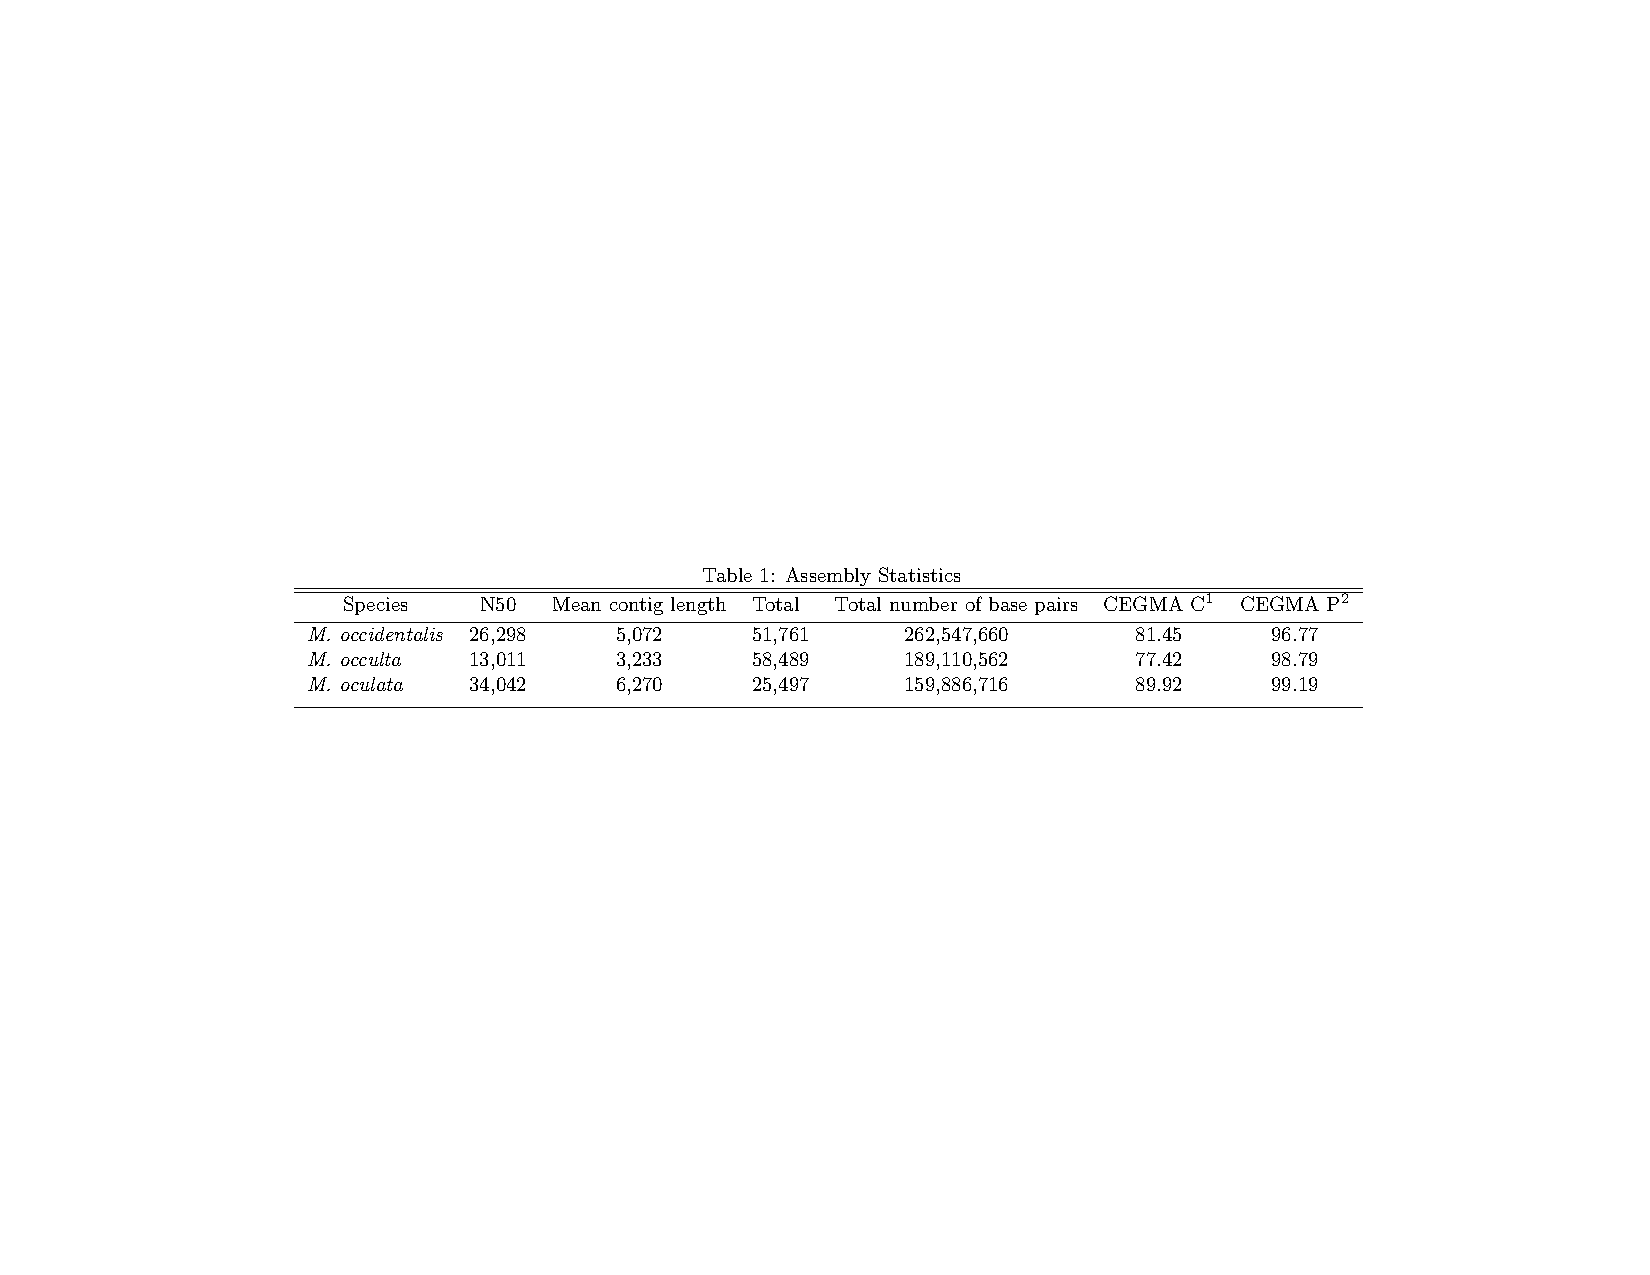
\includegraphics[width=\linewidth]{figures/genome_table_1}
\caption{\textbf{Genome assembly statistics.} The contig N50 length, mean contig length, total number of contigs, total number of base pairs and CEGMA scores were collected for each draft assembly. The CEGMA scores is a metric of completeness measured against highly Conserved eukaryotic genes. Alignments of 70\% or greater of the protein length are called complete (C\textsuperscript{1}) and all other statistically significant alignments are called partial (P\textsuperscript{2}).}
\label{table:genome_table}
\end{table}
In addition to N50 lengths, we also used CEGMA (Core Eukaryotic Genes Mapping Approach) scores, in order to evaluate the assemblies' representative completeness \cite{parra_cegma:_2007}. CEMGA reports scores for complete and partial alignments to a subset of core eukaryotic genes. An alignment is considered ``complete'' if at least 70\% of a given protein model aligns to a contig in the assembly, while a partial alignment indicates that a statistically significant portion of the protein model aligns. The partial alignment scores are \mytilde97\% or higher for all assemblies. \textit{M. oculata} has the best complete alignment score at \mytilde90\%. \textit{M. occidentalis} and \textit{M. occulta} have complete alignment scores of 81\% and 77\% respectively (Table~\ref{table:genome_table}). These scores indicate that our assemblies contain at least partial sequences for the vast majority of protein-coding genes in the genomes of these species.
Various factors make it unreliable to predict genome size and gene density based on assembly metrics alone \cite{bradnam_assemblathon_2013}. Of the handful of sequences we isolated and analyzed, we found that the sizes of introns and upstream regulatory regions were roughly comparable to those from their \textit{Ciona} orthologs. This suggests that the \textit{Molgula} genomes may be as compact as the \textit{C. intestinalis} genome (i.e., \mytilde150-170 Mb, \mytilde16,000 genes, \cite{laird_chromatid_1971,simmen_gene_1998,satou_improved_2008}.

\begin{figure}[tbp]
\centering
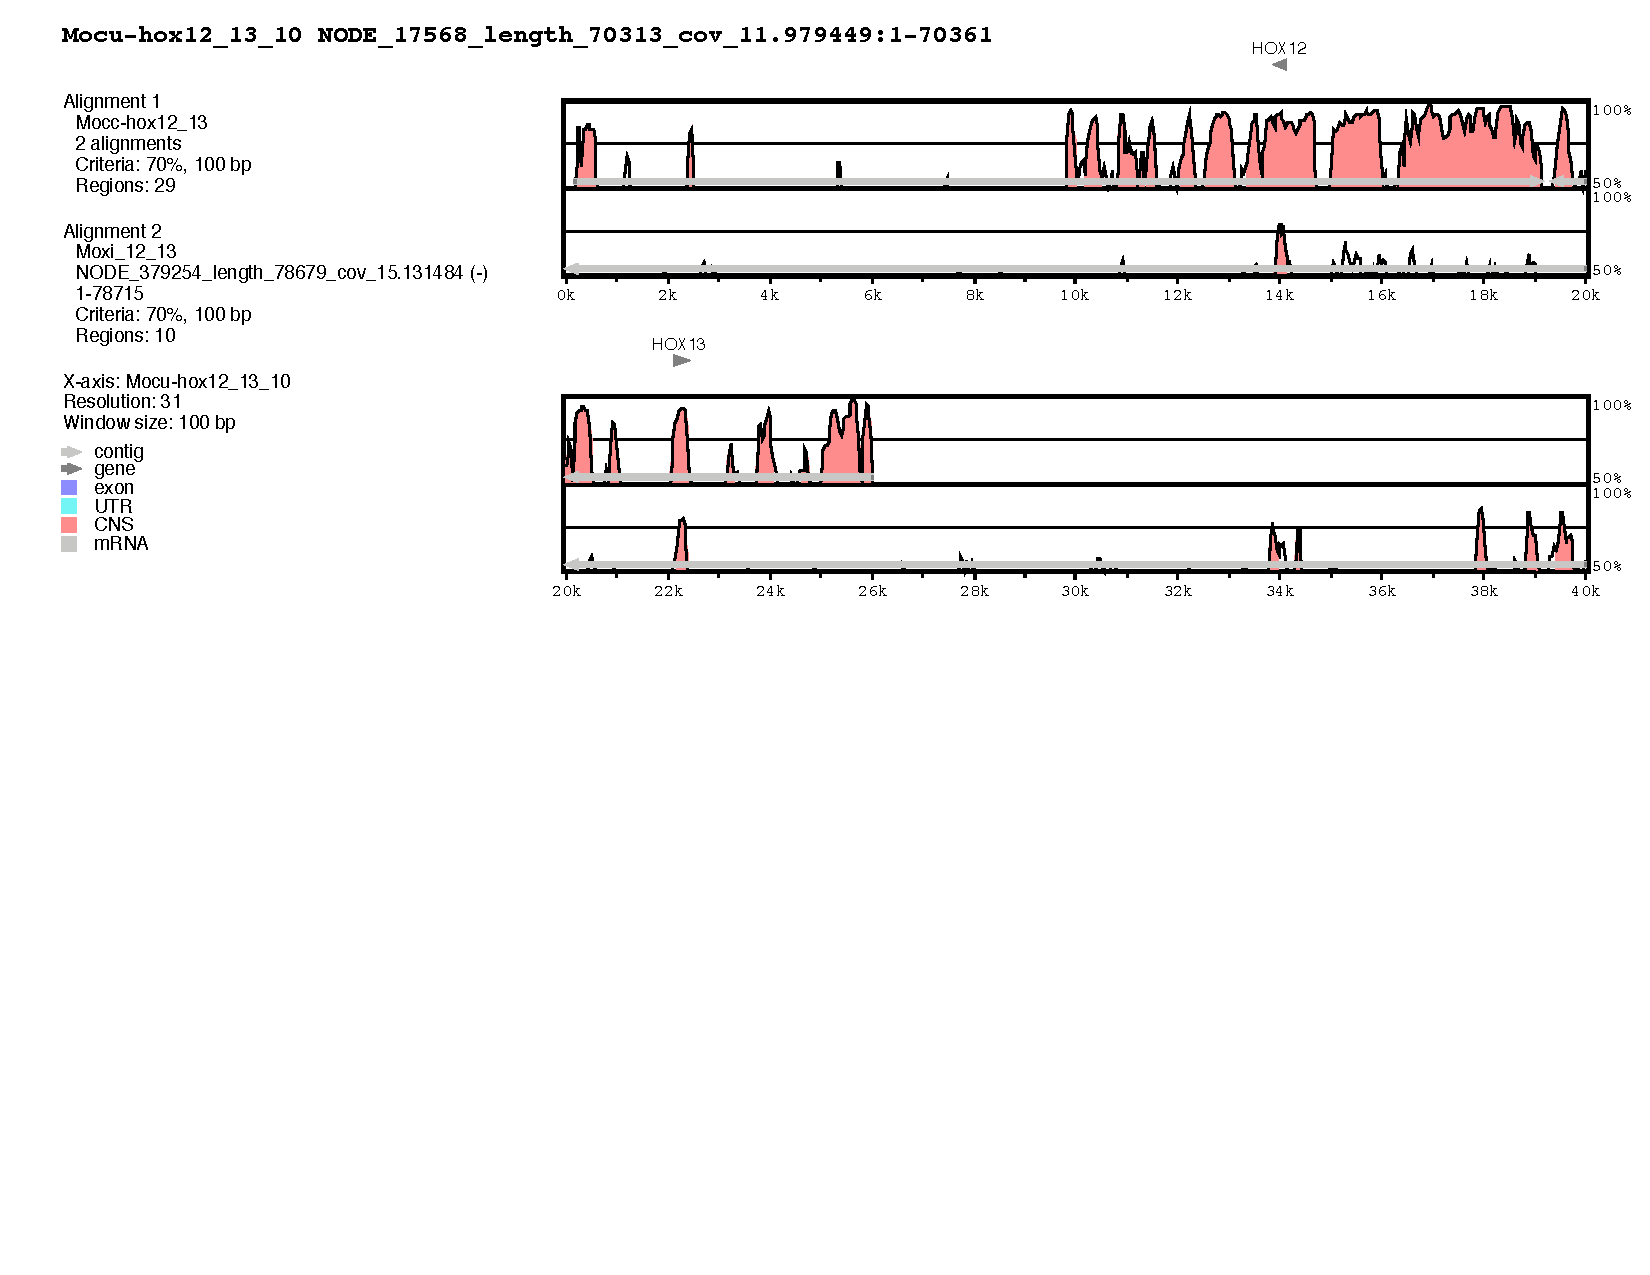
\includegraphics[scale=0.6]{figures/Hox12_13.pdf}
\caption{\textbf{Alignment for \textit{hox12-13} in \textit{M. occulta}, \textit{M. oculata} and \textit{M. occidentalis}} The contig containing \textit{hox12-13} for \textit{M. occidentalis} and \textit{M. oculata}, along with the two contigs containing \textit{hox12} and \textit{hox13} for \textit{M. occulta}. \textit{M. oculata} was used as the anchor sequence because it showed the most similar between the three species. Outside of the coding regions and its flanking area, there is very little sequence similarity, between the species, and \textit{M. occidentalis} exclusively shows similar in coding regions. Grey arrows show the direction of the contig.}
\label{fig:hox12}
\end{figure}
\subsection{Gene complexes}
\textit{Hox} genes are known to be involved with the establishment of morphological identities along the anteroposterior axis of bilaterians and cnidarians \cite{finnerty_origins_2003}. There are 4 \textit{HOX} clusters in humans totaling in 39 genes. Within tunicates, \textit{C. intestinalis}, \textit{Halocythia roretzi} and \textit{Oikopleura dioica} \textit{hox} genes have been characterized. \textit{C. intestinalis} has 9 \textit{hox} genes, \textit{Hox1} through \textit{6}, \textit{Hox10}, and \textit{Hox12-13} \cite{dehal_draft_2002}. The \textit{hox} gene of \textit{C. intestinalis} where initially found on 5 scaffolds spanning \mytilde{980} kb using the draft assembly, with \textit{hox2-4}, \textit{hox5-6} and \textit{hox12-13} being found on the same scaffold.  two clusters of hox genes across two chromosomes \cite{ikuta_ciona_2004}. \textit{O. dioica} also has 9 hox genes, hox1-2, hox4, a duplicate hox9, and hox10-13, however, none of the genes have been found on the same scaffold, even using a 250 kb window \cite{siok_biological_2004}. Eight \textit{hox} genes have be found in \textit{M. occulta} and \textit{M. oculata}, while nine have been found in \textit{M. occidentalis}. \textit{Hox1}, \textit{hox2}, \textit{hox3-4}, \textit{hox5}, \textit{hox10} and \textit{hox12-13}, with \textit{hox3-4} being found on the same contig in all three species. Additionally \textit{hox10}, and \textit{hox12-13} are found on the same contig in \textit{M. oculata} with only \textit{hox12-13} being found on the same contig in \textit{M. occidentalis}. However, it appears that the \textit{hox} genes have been rearranged in \textit{M. oculata}, \textit{hox10} is downstream of \textit{hox12-13}. \textit{Hox12-13} are not found on the same contig in \textit{M. occulta}, however when aligned with mVista there appears to be a strong case for synteny (Figure~\ref{fig:hox12}). \textit{M. occidentalis} had one additional \textit{hox} gene compared to \textit{M. occulta} and \textit{M. oculata}, there appears to be a duplicate \textit{hox10} gene \mytilde12kb apart found on the same contig. \textit{M. occulta}, \textit{M. oculata}, and \textit{M. occidentalis hox} genes span across 7, 6 and 5 contigs respectively and spends xxx kb, 333 kb and sass kb, respectively.  This show to be more compact that \textit{Ciona} which spends 3\textit{x} as many base pair, but these show to be 3x that of human. hox2 has a stop codon located in the 3-4 helix. 

how similar the hox10 duplicate is in oxi

There is very little synteny between M. occulta, M. oculata and M. occidentalis. When looking at the hox complex for both hox3-4 and hox12-13, only in coding regions does there appear to be syntyany.  

Ciona exhibits longer and than usual introns between hox genes, averaging in the 5Mb range, when typically the hox genes have 100-120 kb separating them \cite{mcginnis_homeobox_1992}
Because of the lack of homology outside of coding regions, we were able to identify distaless location downstream of hox13 in both M. occidentalis and M. oculata, this was not the case for M. occulta. 
\begin{figure}[tbp]
\centering
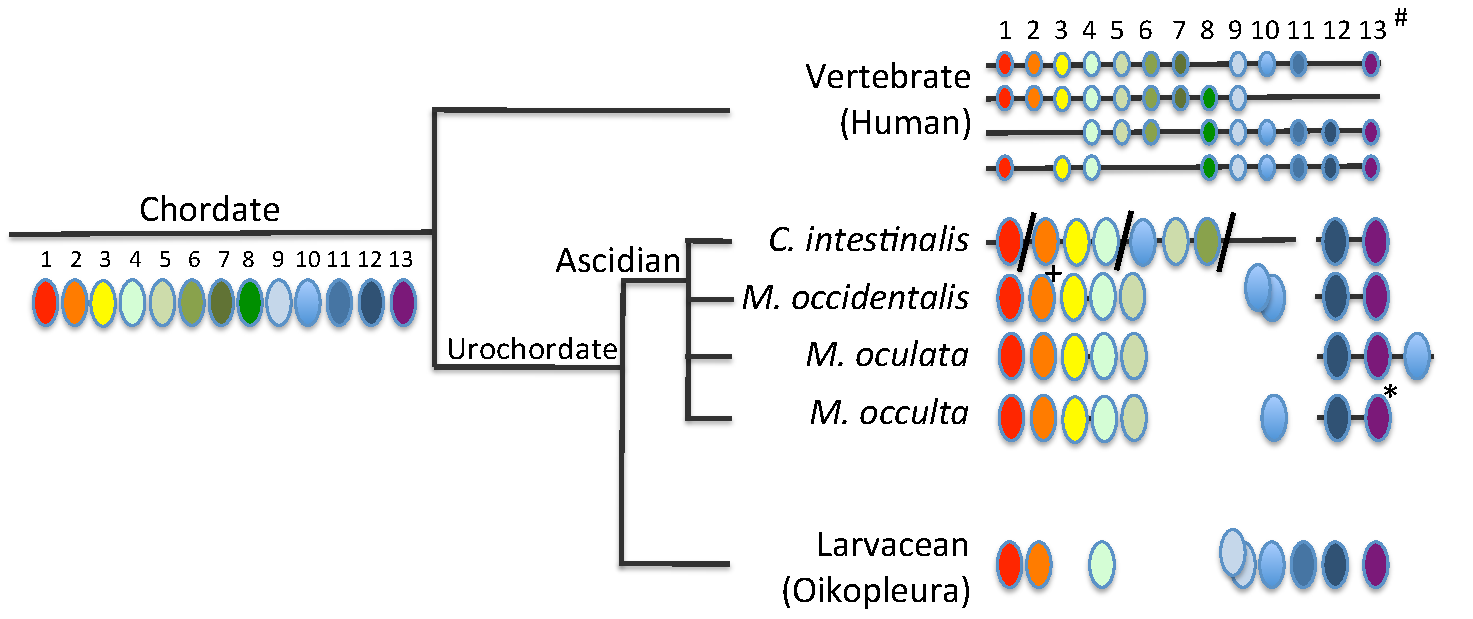
\includegraphics[scale=0.65]{figures/hox.pdf}
\caption{\textbf{Hox clusters for \textit{M. occulta}, \textit{M. oculata} and \textit{M. occidentalis}} Eight \textit{hox} genes were found in  \textit{M. occulta} and \textit{M. oculata}, while nine were found in \textit{M. occidentalis}. \textit{Hox1}, \textit{hox2}, \textit{hox3-4}, \textit{hox5}, \textit{hox10} and \textit{hox12-13} were found in all three \textit{Molgula} species. \textit{Hox3-4} were found on the same contig in all species, with \textit{hox12-13} being found on the same contig in \textit{M. occidentalis} and \textit{M. oculata}. *\textit{M. occulta} \textit{hox12-13} are not found on the same contig, but when aligned using mVista, this is high sequence similar, showing the possible placement for of \textit{hox12-13} in \textit{M. occulta}. \textsuperscript{+}\textit{M. occidentalis} \textit{hox2} gene had a stop codon found in the 3-4 helix. \textsuperscript{\#} numbers correspond to gene color, rearrangement has be found in \textit{Ciona} and \textit{Molgua}.}
\label{fig:hox12}
\end{figure}
\subsection{Divergence of GRN}
Our sequencing efforts revealed extreme genetic divergence not only between \textit{Ciona} and \textit{Molgula}, as expected, but even within the Molgulids. For example, we used BLAST to identify the \textit{Molgula} orthologs of \textit{C. intestinalis Mesp} (\textit{Ciinte.Mesp}, as per the proposed tunicate gene nomenclature rules, see Stolfi et al., \cite{stolfi_guidelines_2014}). \textit{Ciinte.Mesp} is the sole ortholog of vertebrate genes coding for \textit{MesP} and \textit{Mesogenin bHLH} transcription factor family members \cite{satou_improved_2008}. VISTA alignment shows high sequence similarity between sequences 5' upstream of the \textit{Mesp} genes from the closely related \textit{M. oculata} and \textit{M. occulta} (Figure 1B). However, there is no conservation of \textit{Mesp} DNA sequences, coding or non-coding, between \textit{M. oculata}/\textit{occulta} and \textit{M. occidentalis}, nor between \textit{C. intestinalis} and any of the three \textit{Molgula} species (Figure 1?figure supplement 1). In previous phylogenetic surveys, \textit{M. occidentalis} has been placed as an early-branching \textit{Molgula} species, often grouped together in a subfamily with species ascribed to the genera Eugyra and Bostrichobranchus instead \cite{hadfield_multiple_1995,huber_evolution_2000,tsagkogeorga_updated_2009}. Our sequencing results support the view that \textit{M. occidentalis} is highly diverged from other \textit{Molgula} spp.
This sequence divergence was also evident when analyzing the \textit{hox} genes. When comparing sequence similarity of the \textit{hox} genes that were found on the same contigs, only regions clustered around the coding region for \textit{M. occulta} when compared to \textit{M. oculata}, and only coding sequences showed similarity in \textit{M. occidentalis}. 

\section{Discussion and Conculsion}
Three \textit{Molgula}\textemdash\textit{M. occulta}, \textit{M. oculata} and \textit{M. occidentalis}\textemdash species have been sequenced and assembled, this is the first of any molgulides to have assembled genomes. Developmentally the three species are very similar up to the gastrula stage, where \textit{M. occulta} diverge from the typical solitary ascidian body plan and develops without a tail. In vertebrate the hox patterning has shown to be an important some or another. The same has not be shown in ascidans, \textit{hox} has more of a tissue specific role in ascidians. It is proposed that ascidians evolved there simple body plans and rapid embryogensis through extensive genomeic rearrangement and gene loss, some of those genes being hox genes\cite{ikuta_organization_2005}. \textit{Ciona} has 10 \textit{hox} genes and is missing hox7-9 and 11. \textit{Hox6} is miss from all three species, which is not surprising that the \textit{Molugla} have loss \textit{hox6}, which is also missing in \textit{O. dioica} and no express has been about to be detected in \textit{C. intestinalis} through Whole Mount In Situ Hybridization at any stages of development \cite{ikuta_ciona_2004}. No two of the \textit{Molgula} species show the same \textit{hox} pattern and show a strong divergence outside of coding regions, even more so in \textit{M. occidentalis}. There is a duplicate in \textit{Mocci.hox10} which could lead to a split in function seeing that is \textit{Ciinte.Hox10}  expressed in to region during the mid-tailbud stage\textemdash a small region of anterior the nerve cord, and a small area of the posterior ventral endoderm and adjacent tissue\cite{ikuta_ciona_2004}.